In leading order we have to consider photon-gluon-fusion (PGF), that is
\begin{equation}
\Pggx(q) + \Pg(k_1) \rightarrow \PQ(p_1)+\PaQ(p_2)
\end{equation}
with two contributing diagrams depicted in figure \ref{fig:FeynLO}.
\begin{figure}[ht!]
\centering
\begin{subfigure}[t]{.4\textwidth}
	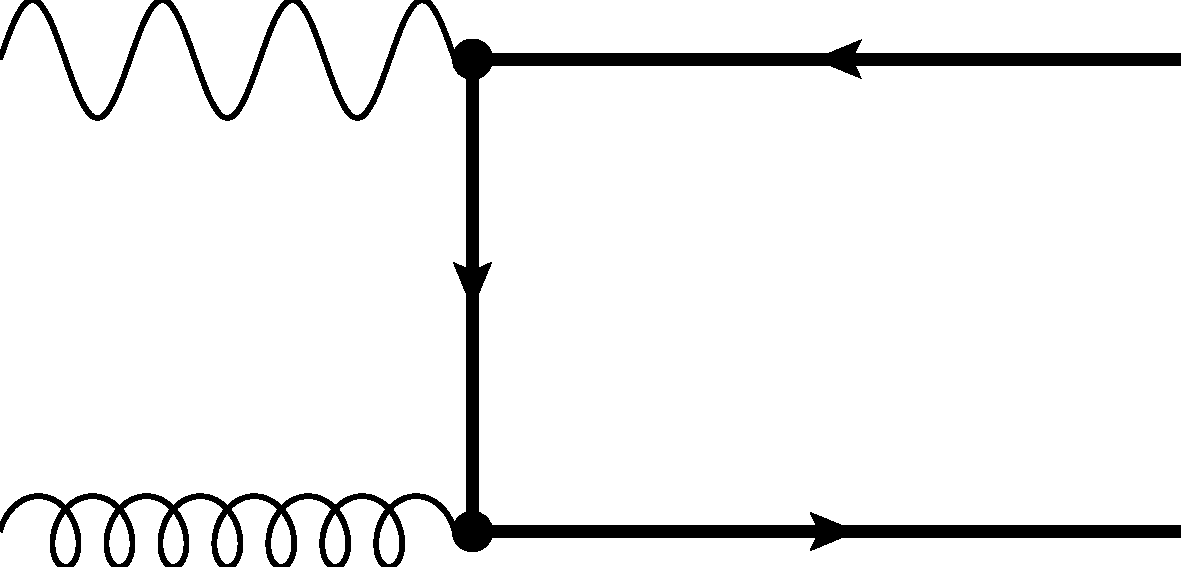
\includegraphics[width=\textwidth]{pyfeyn/lo-1}
	\caption{$i\varepsilon^{\mu}_{\Pgg}(q)\varepsilon^{\nu}_{\Pg}(k_1)\Md^{(0),1}_{\mu\nu}$}
\end{subfigure}\hspace{.15\textwidth}%
\begin{subfigure}[t]{.4\textwidth}
	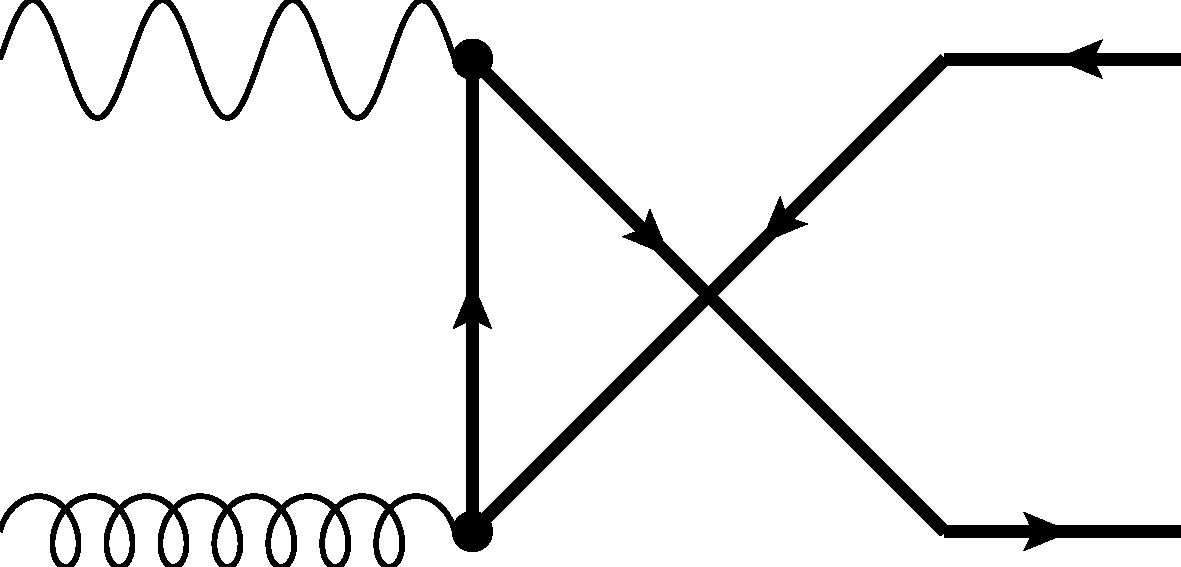
\includegraphics[width=\textwidth]{pyfeyn/lo-2}
	\caption{$i\varepsilon^{\mu}_{\Pgg}(q)\varepsilon^{\nu}_{\Pg}(k_1)\Md^{(0),2}_{\mu\nu}$}
\end{subfigure}
\caption{leading order Feynman diagrams}\label{fig:FeynLO}\fxerror{shift to appendix?}
\end{figure}

The result can then be written as
\begin{equation}
\hat {\mathcal P}_{\vec k}^{\Pgg,\mu\mu'}\hat {\mathcal P}_{\vec k}^{\Pg,\nu\nu'}\sum_{j,j'=1}^2\Md^{(0),j}_{\mu\nu}\left(\Md^{(0),j'}_{\mu'\nu'}\right)^* = 8g^2\mu_D^{-\epsilon}e^2e_H^2 N_C C_F B_{\vec k,QED}
\end{equation}
where $g$ and $e$ are the strong and electromagnetic coupling constants respectively, $\mu_D$ is an arbitray mass parameter introduced to keep the couplings dimensionless and $e_H$ is the magnitude of the heavy quark in units of $e$. Further $N_C$ corresponds to the gauge group $SU(N_C)$ and the color factor $C_F=(N_C^2-1)/(2N_C)$ refers to the second Casimir constant of the fundamental representation for the quarks. We then find:
\begin{align}
B_{\tVV,F_2,\tQED} &= -1 - 6\frac{q^2}{s'} - 6\frac{q^4}{{s'}^2} + \frac{q^2(6m^2+s) +2m^2 s + s'^2/2}{t_1u_1} - \frac{(2m^2+q^2)m^2s'^2}{(t_1 u_1)^2}\nonumber\\
 &\hspace{20pt}+\frac{\epsilon}{2}\left\{ -1 + \frac{s^2-q^2s'}{t_1u_1} - \frac{m^2q^2{s'}^2}{t_1^2u_1^2} \right\} + \epsilon^2\frac{{s'}^2}{8t_1u_1}\\
B_{\tVV,F_L,\tQED} &= -\frac{4q^2}{s'}\left(\frac s {s'} - \frac{m^2s'}{t_1u_1}\right)\\
B_{\tVV,2xg_1,\tQED} &= \\
B_{\vec k,\tQED} &= B^{(0)}_{\vec k,\tQED} + \epsilon B^{(1)}_{\vec k,\tQED} + \epsilon^2 B^{(2)}_{\vec k,\tQED}
\end{align}

